\providecommand{\atd}{..}
\documentclass[../main.tex]{subfiles}

\begin{document}
    \chapter{SWOT Analysis}
    \section{Template}
    \begin{figure}[H]
        \centering
        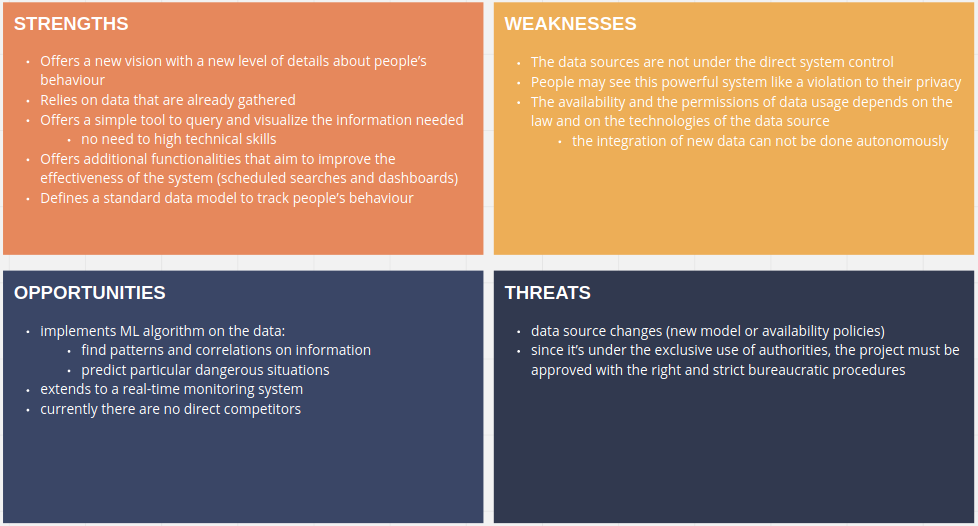
\includegraphics[scale = 0.5]{assets/swot.png} \\
        \caption[]{Swot Analysis template}\label{fig:figure10}
    \end{figure}
    \chapter{Promises and Potentials Map}
    \section{Template}
    \begin{figure}[H]
        \centering
        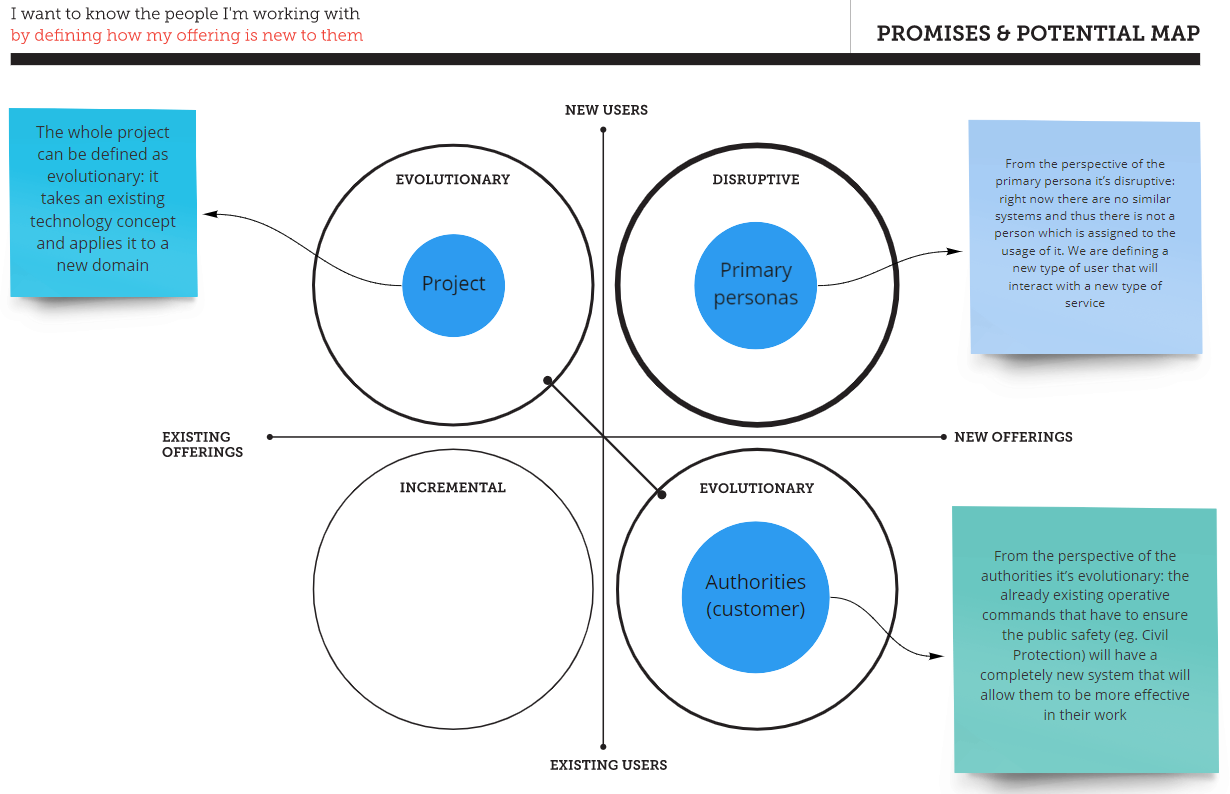
\includegraphics[scale = 0.4]{assets/promises.png} \\
        \caption[]{Promises and Potentails Map Template}\label{fig:figure11}
    \end{figure}
    \chapter{General representation of the company}
    Central Safety System s.r.l. is a PMI Innovativa (PMII) an italian company type for small and medium companies.
    Born as a startup around the main idea to take advantage of multiple already existing data sources for security purpose that evolved into the project “Central Safety System”.
    After pre-seed and seed rounds our idea became our product, around which we have founded Central Safety System s.r.l.
    Our first main client is Italian Civil Protection of Milan and the plan is to expand the usage of Central Safety System to Italian Civil Protection in any region.
    A market segment of potential customers that could benefit from our product, that have the same needs to which our product is aligned.
    In our company stage defining our focusing in terms of features is vital because, without it, potential users who have divergent needs could pull our product in many different directions.

    \section{Company Structure}
    \subsection{Description}
    The company structure is divided in four main departments:
    \begin{itemize}
        \item \textbf{Legal department}: which is responsible to the legal aspects of the projects and the supervision of the data protection strategy. Since the system relies on external already-existing data sources, the legal and bureaucratic definition on how the data are accessed, gathered, stored and used are key points.
        \item \textbf{Sale Department}: which is in charge to manage sales and relationships with clients and new ones. Initially the target customers are clearly defined: the Italian Civil Protection, or in general an authority that is in charge of ensure the public safety. The sales department is perhaps focused and skilled in dealing with Public Administration entities.
        \item \textbf{Technical support \& Training departments}:  it manages everything from the deploy and installation of the system to the training of employees of our customers, technical support and fix opened tickets. Since our project is a completely new product, we can exploit business opportunities also in offering training course (and potentially certification) to the customers.
        \item \textbf{Development Department}: which is divided in two distinct teams:
        \begin{itemize}
            \item \textit{Project Team}: works on the development of new features on our product Central Safety System. The project team can focus only on the data model and the operation that our system perform on it (analysis, searches, visualizations…) without worrying about how the data are gathered.
            \item \textit{ETL Team}: works on how to integrate data from multiple sources. Given a source and the accesses methodologies (there should be a strict collaboration with the legal department in this stage), the team is able to define queries and scripts that allow to extract the data and transform them in order to made the information consistent with our data model.
        \end{itemize}
    \end{itemize}
    \textbf{Outsourced department}:
    \textit{Marketing department}: due to the fact that we are a B2B company we do not need an internal department focused on marketing. A possible marketing campaign strictly related to our product can aim to reassure citizens about the system purpose and the contribution that gives to the public safety.

    \subsection{Template}
    \begin{figure}[H]
        \centering
        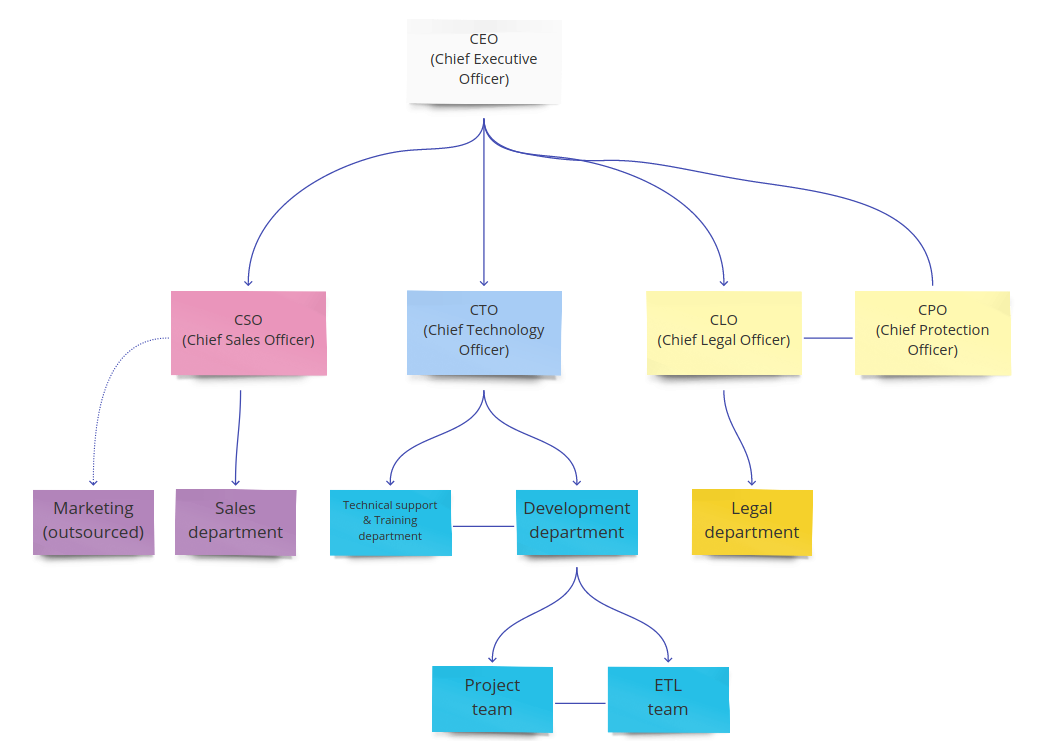
\includegraphics[scale = 0.5]{assets/company.png} \\
        \caption[]{Company Structure}\label{fig:figure13}
    \end{figure}
    \newpage
    \section{Data Management}
    Nowadays data protection and management is highly regulated by the GDPR General Data Protection Regulation (Regulation (EU) 2016/679).\\
    \textbf{GDPR} specifies how personal data should be lawfully processed (including how it’s collected, used, protected or interacted with in general).
    It requires that both data controllers and data processors keep and maintain “full and extensive” up-to-date records of the particular data processing activities they are carrying out.\\
    \textbf{Data Protection Officer (DPO)}: GDPR requires designation of a DPO specifically where the processing is carried out by a public authority (except for courts or independent judicial authorities).
    Data protection officers are responsible for the supervision of the data protection strategy and implementation in order to ensure compliance with statutory requirements.

    \section{Integration}
    The integration of a new software with others already existing is a crucial key point in nowadays companies.
    However, we have to consider two main aspects:
    \begin{itemize}
        \item Our customers will be authorities, which are different from “typical” business companies.
        \item Our product is a completely new system which does not expect external integration but the data sources. In fact, all the data gathered are confidential and at exclusive use of the authorities and to date there are no reasons to implement integration with other services.
    \end{itemize}
    Nevertheless, since our customers are really similar, have the same needs and potentially relies on the same structures, the possibilities of integration between our software and other services is actually possible without too much effort.
    Now we will illustrate how our product integrates with two type of system (a CRM and a Recommender), please notice that:
    \begin{itemize}
        \item Those services have no access to the data or to the functionalities offered by our system.
        \item They cannot be considered as “external already existing softwares”, since the integration is fully managed by our development team.
    \end{itemize}

    \section{Enterprise Architecture}
    \subsection{Description of Zachman Framework}
    Each cell of the Zachman Framework below, is composed either by a textual description or by mentioning a diagram previously built during the deliverables.
    Where the diagrams were missing, we made some hypothesis on what that cell should have contained:
    \begin{itemize}
        \item \textit{ER Diagram}: describes interrelated things of interest in a specific domain of knowledge. A basic ER model is composed of entity types (which classify the things of interest) and specifies relationships that can exist between entities (instances of those entity types).
        \item \textit{Logistics Network}: The sequence or system of organizations or operations that work together to design, produce, and deliver a product or service to a market, extending from the extraction of raw materials to the distribution of finished products or services.
        \item \textit{Master Schedule}: a plan for individual commodities to be produced in each time period such as production, staffing, inventory, etc.
        \item \textit{Business Plan}: a formal written document containing business goals, the methods on how these goals can be attained, and the time frame within which these goals need to be achieved.
        \item \textit{UML Diagram}: a diagram based on the UML (Unified Modeling Language) with the purpose of visually representing a system along with its main actors, roles, actions, artifacts or classes, in order to better understand, alter, maintain, or document information about the system.
        \item \textit{Data Flow Diagram}: a way of representing a flow of data through a process or a system (usually an information system). The DFD also provides information about the outputs and inputs of each entity and the process itself.
        \item \textit{Distributed Systems Architecture}: composed of various hardware and software (collectively called components) that communicate with each other only by transfer of messages.
        \item \textit{Workflow Model}: is the sequential series of tasks and decisions that make up a business process.
        \item \textit{Entity Life History}: is a diagrammatic method of recording how information may change over time, and models the complete catalogue of events that can affect a data entity from its creation to its deletion, the context in which each event might occur, and the order in which events may occur.
        \item \textit{Business Rule Model}: to specify requirements for application software.
        \item \textit{Control Flow Diagram}: is a diagram to describe the control flow of a business process, process or review.
        \item \textit{System Architecture}: is the conceptual model that defines the structure, behavior, and more views of a system.
    \end{itemize}
    \subsection{Zachman Framework Template}
    \begin{figure}[H]
        \centering
        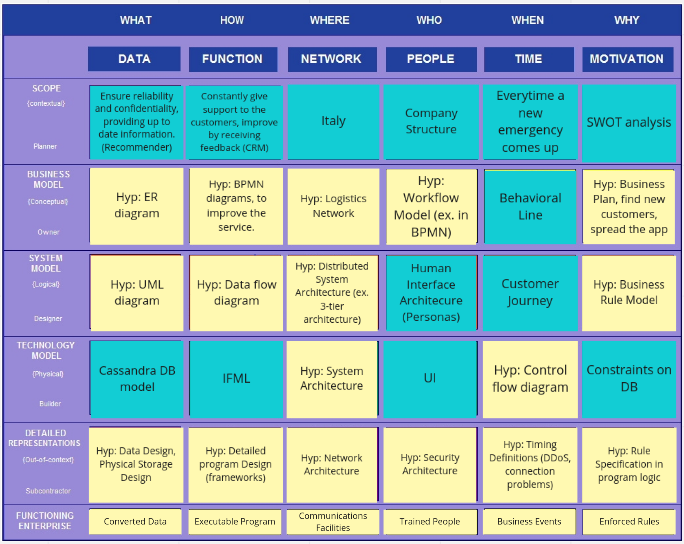
\includegraphics[scale = 0.5]{assets/zachman.png} \\
        \caption[]{Zachman Framework}\label{fig:figure12}
    \end{figure}
    \newpage
    \section{CRM}
    Our company will surely rely on a CRM to handle customers. However we have to consider the types of customers that will interact with our one-product company (at least for now). In fact, we won’t have to handle a product that will be adopted by a very large amount of people like a mobile application or a social network because our system is at exclusive use of authorities.
    The main advantage that we can obtain from the integration with a CRM is the possibility to get in touch with the customers in order to:
    \begin{itemize}
        \item Receive feedbacks
        \item Offer Support
    \end{itemize}
    Since our product is a completely new kind of system that is addressed to a new kind of users, the possibility to receive constant feedback can help the the development of the system and set the right direction for the future features.
    In addition, our company will take care of the support and the training session offered to the customers. A direct integration of the CRM with the company information system can ensure the right effectiveness in handling the customer requests and exploit the business opportunities of support and training.
    It should be possible also to integrate a communication channel directly in the product: something like a chat, a contact form or a “ticket” system that interfaces directly with the CRM.

    \section{Recommender System}
    A recommender system can be integrated in our product. The main challenge is to find an effective way to collect the interaction of the users with the system: the filters used, the executed searches, the refinement made after a search…
    Perhaps, our recommender system should be able to find patterns among user interaction and be able to recommend the filters to set for a certain search or to obtain a particular effective visualization.
    The methods used by this recommender system can be:
    \begin{itemize}
        \item Association rules: for example, which kind of visualization is used when certain filters are set
        \item Collaborative filtering: suggest the refinement of a search based on other users that made similar searches
    \end{itemize}
    Since the recommender relies on the user interactions and not on the data gathered by our product, we can share the information used for prediction among all the instances. Having more information on which we compute our recommendation will surely increase the possibility to make useful suggestion. In addition, the gathered data about interactions represents a sort of knowledge base on how our product is actually used.

    \section{Database Model}
    \subsection{DB Description}
    The database solution we opted for is the column-oriented database Cassandra.
    The immediate availability and the speed of the query operations make it the optimal solution for the analysis on the large quantities of heterogeneous data that the system collects. Once the exponential phase of data collection has been overcome, the linear growth of the size of the system would occur in the presence of many GB of records; for this reason the solution must support a heavy load of write operations. Furthermore, the elastic scalability makes Cassandra the optimal approach in the cloud environment, the target development environment of the system. Considering the data model, the fluid data structure of the column-oriented approach removes any constraint for the development of new features that involve the use of additional data not previously existing. Being our product in continuous evolution, this need must be satisfied in order to have a flexible structure that easily adapts to fast software evolutions.

    The model described in the diagrams below was created by abstracting the use cases in the various analysis and monitoring scenarios that the platform manages. The correspondence is particularly evident if we consider the interactions described in the wireframes, in which the setting of the filters corresponds to a query event generated according to a predefined scheme.

    \subsection{DB Templates}
    \begin{figure}[H]
        \centering
        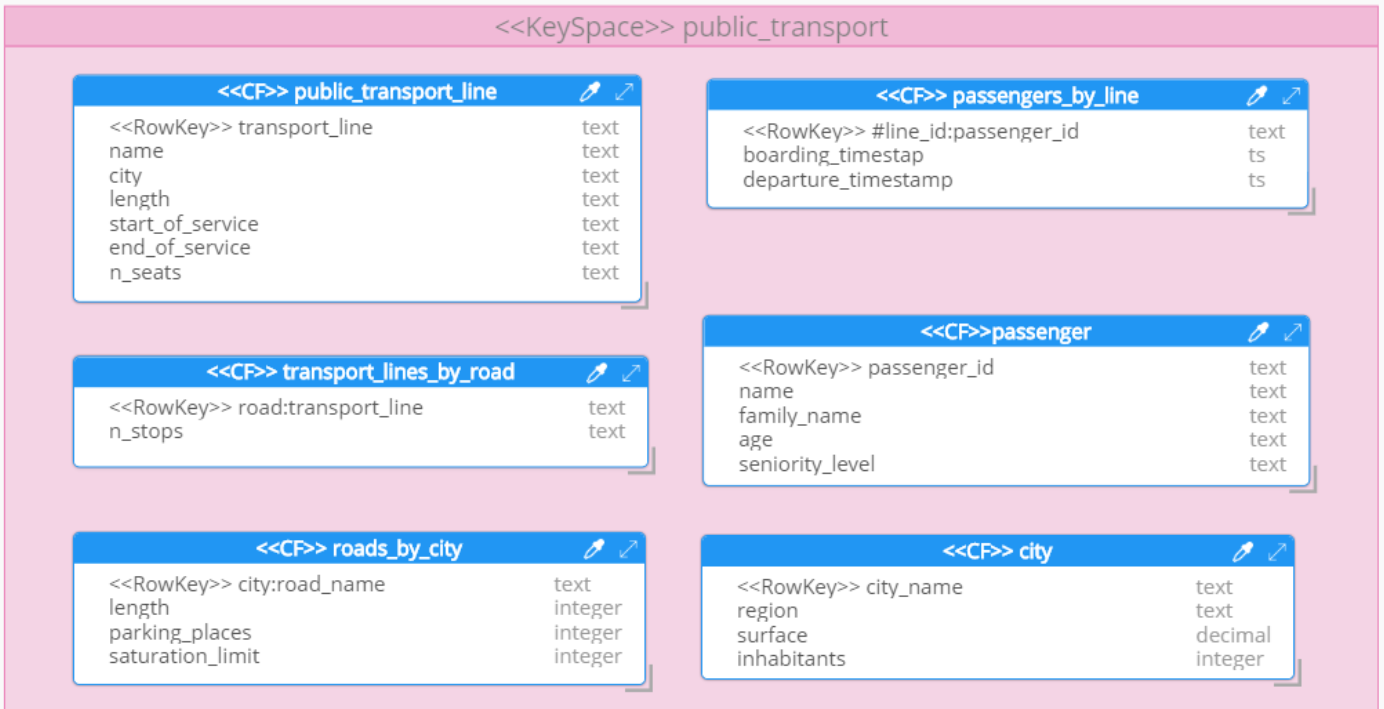
\includegraphics[scale = 0.6]{assets/db/cassandra_1.png} \\
        \caption[]{Public Transport DB}\label{fig:figure14}
    \end{figure}
    \begin{figure}[H]
        \centering
        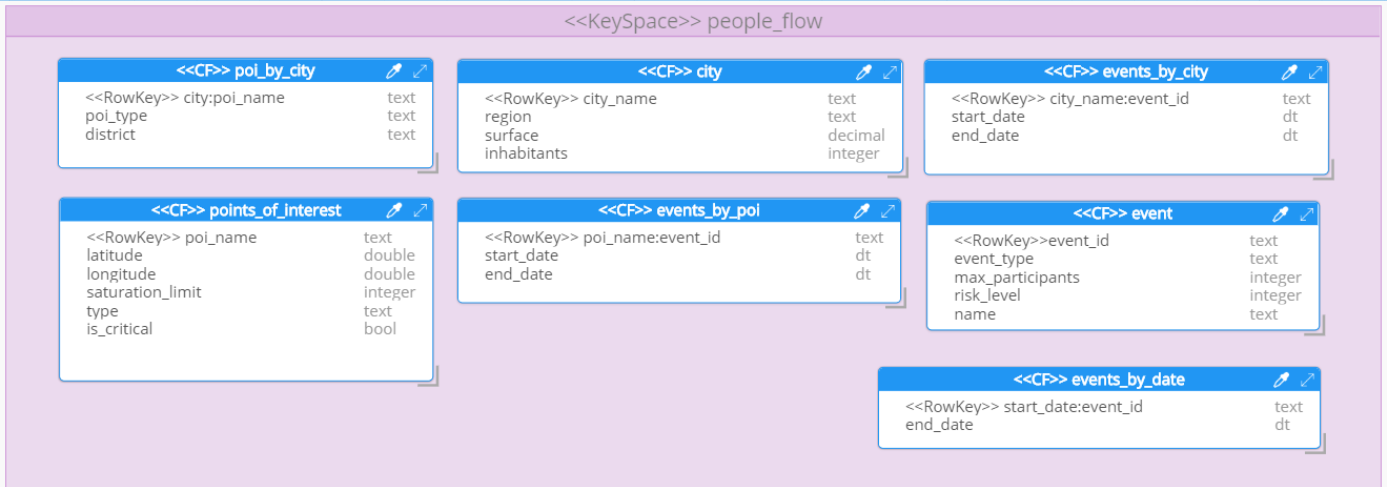
\includegraphics[scale = 0.6]{assets/db/cassandra_2.png} \\
        \caption[]{People Flow DB}\label{fig:figure15}
    \end{figure}
    \begin{figure}[H]
        \centering
        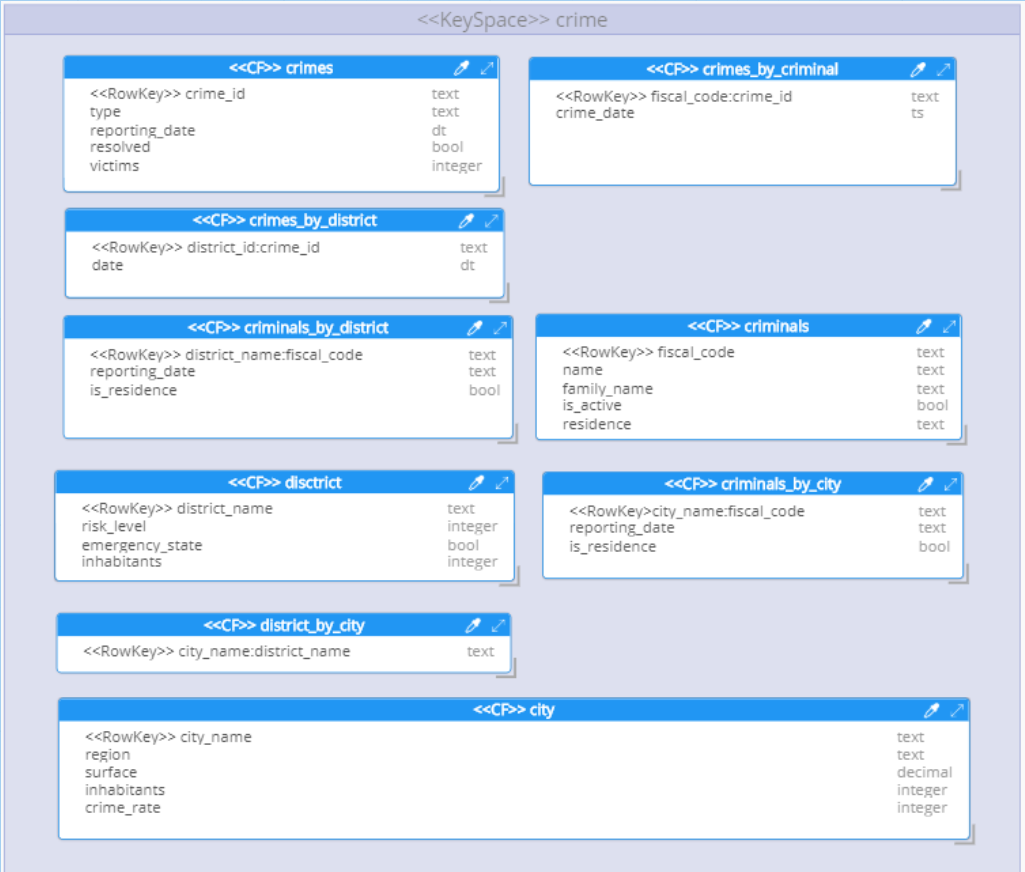
\includegraphics[scale = 0.8]{assets/db/cassandra_3.png} \\
        \caption[]{Crimes DB}\label{fig:figure16}
    \end{figure}



\end{document}